\documentclass[titlepage]{jsarticle}
\usepackage[dvipdfmx]{graphicx}
\usepackage{listings}
\usepackage{h31ec-exp}
\usepackage{biblatex}
\lstset{
  basicstyle={\ttfamily},
  identifierstyle={\small},
  commentstyle={\smallitshape},
  keywordstyle={\small\bfseries},
  ndkeywordstyle={\small},
  stringstyle={\small\ttfamily},
  frame={tb},
  breaklines=true,
  columns=[l]{fullflexible},
  numbers=left,
  xrightmargin=0zw,
  xleftmargin=3zw,
  numberstyle={\scriptsize},
  stepnumber=1,
  numbersep=1zw,
  lineskip=-0.5ex
}
\renewcommand{\lstlistingname}{ソースコード}
\makeatletter
\newcommand{\figcaption}[1]{\def\@captype{figure}\caption{#1}}
\newcommand{\tblcaption}[1]{\def\@captype{table}\caption{#1}}
\makeatother
\title{シーケンサによる自動制御}
\grade{3年32番}
\author{平田 蓮}
\team{第4班}
\date{2019年12月17日}
\expdate{2019年12月23日, 1月6日, 1月20日}
\coauthor{}

\begin{document}
\maketitle
\section{目的}
  プログラマブルコントローラ(シーケンサ)による自動制御法(リレーラダー方式, ステップラダー方式)を学び, 課題実験のシステムの設計, 確認実習を行うことで理解を深める.
\section{クイズの解答表示システムの設計}
  次節に述べる仕様を満たすプログラムを作成する.
  \subsection{制御仕様}
    \begin{itemize}
      \item 司会者の出題するクイズに対して, もっとも早くボタンを押したデスクのランプを点灯させる.
        点灯後は司会者が押しボタン$PB_4$を押すまで点灯している.
        ただし, 子供チームの押しボタン$PB_{11}$と$PB_{12}$はどちらも押してもランプ$L_1$を点灯させることができるよう,
        有利になっている. また, 博士チームの押しボタン$PB_{31}$と$PB_{32}$は両方とも押さなければランプ$L_3$は
        点灯しないよう, 不利になっている.
      \item 司会者がスイッチSWをONにしたときに, 10秒以内に回答者のランプがついた場合, 電磁石SOLが働いてくす玉が
        割れるようなラッキーチャンスとなる.
        割れたくす玉はラッキーチャンスが終わった後もその状態を保持し, 押しボタン$PB_4$を押すともとに戻る.
    \end{itemize}
  \subsection{設計}
    表\ref{tab:taiou}に上で示したボタン等とシーケンサのゲート番号との対応表,
    図\ref{fig:quiz_lad}, 表\ref{tab:quiz_code}に設計したリレーラダー図, また, それのコーディングを示す.
    \begin{table}[h]
      \caption{入出力対応表}
      \label{tab:taiou}
      \centering
      \begin{tabular}{c|c|c||c|c|c}
        \hline
        記号 &       名前 &             シーケンサ & 記号 &   名前 &            シーケンサ \\ \hline \hline
        $PB_{11}$ & 子供チームのボタン1 & X400 &     $L_1$ & 子供チームのランプ & Y431 \\
        $PB_{12}$ & 子供チームのボタン2 & X401 &     $L_2$ & 学生のランプ      & Y432 \\
        $PB_2$ &    学生のボタン &       X402 &     $L_3$ & 博士チームのランプ & Y433 \\
        $PB_{31}$ & 博士チームのボタン1 & X403 &     SW &    司会者用スイッチ   & X406 \\
        $PB_{32}$ & 博士チームのボタン2 & X404 &     SOL &   くす玉の電磁石    & Y434 \\
        $PB_4$ &    司会者用ボタン &     X405 & & & \\ \hline
      \end{tabular}
    \end{table}
    \begin{figure}[h]
      \centering
      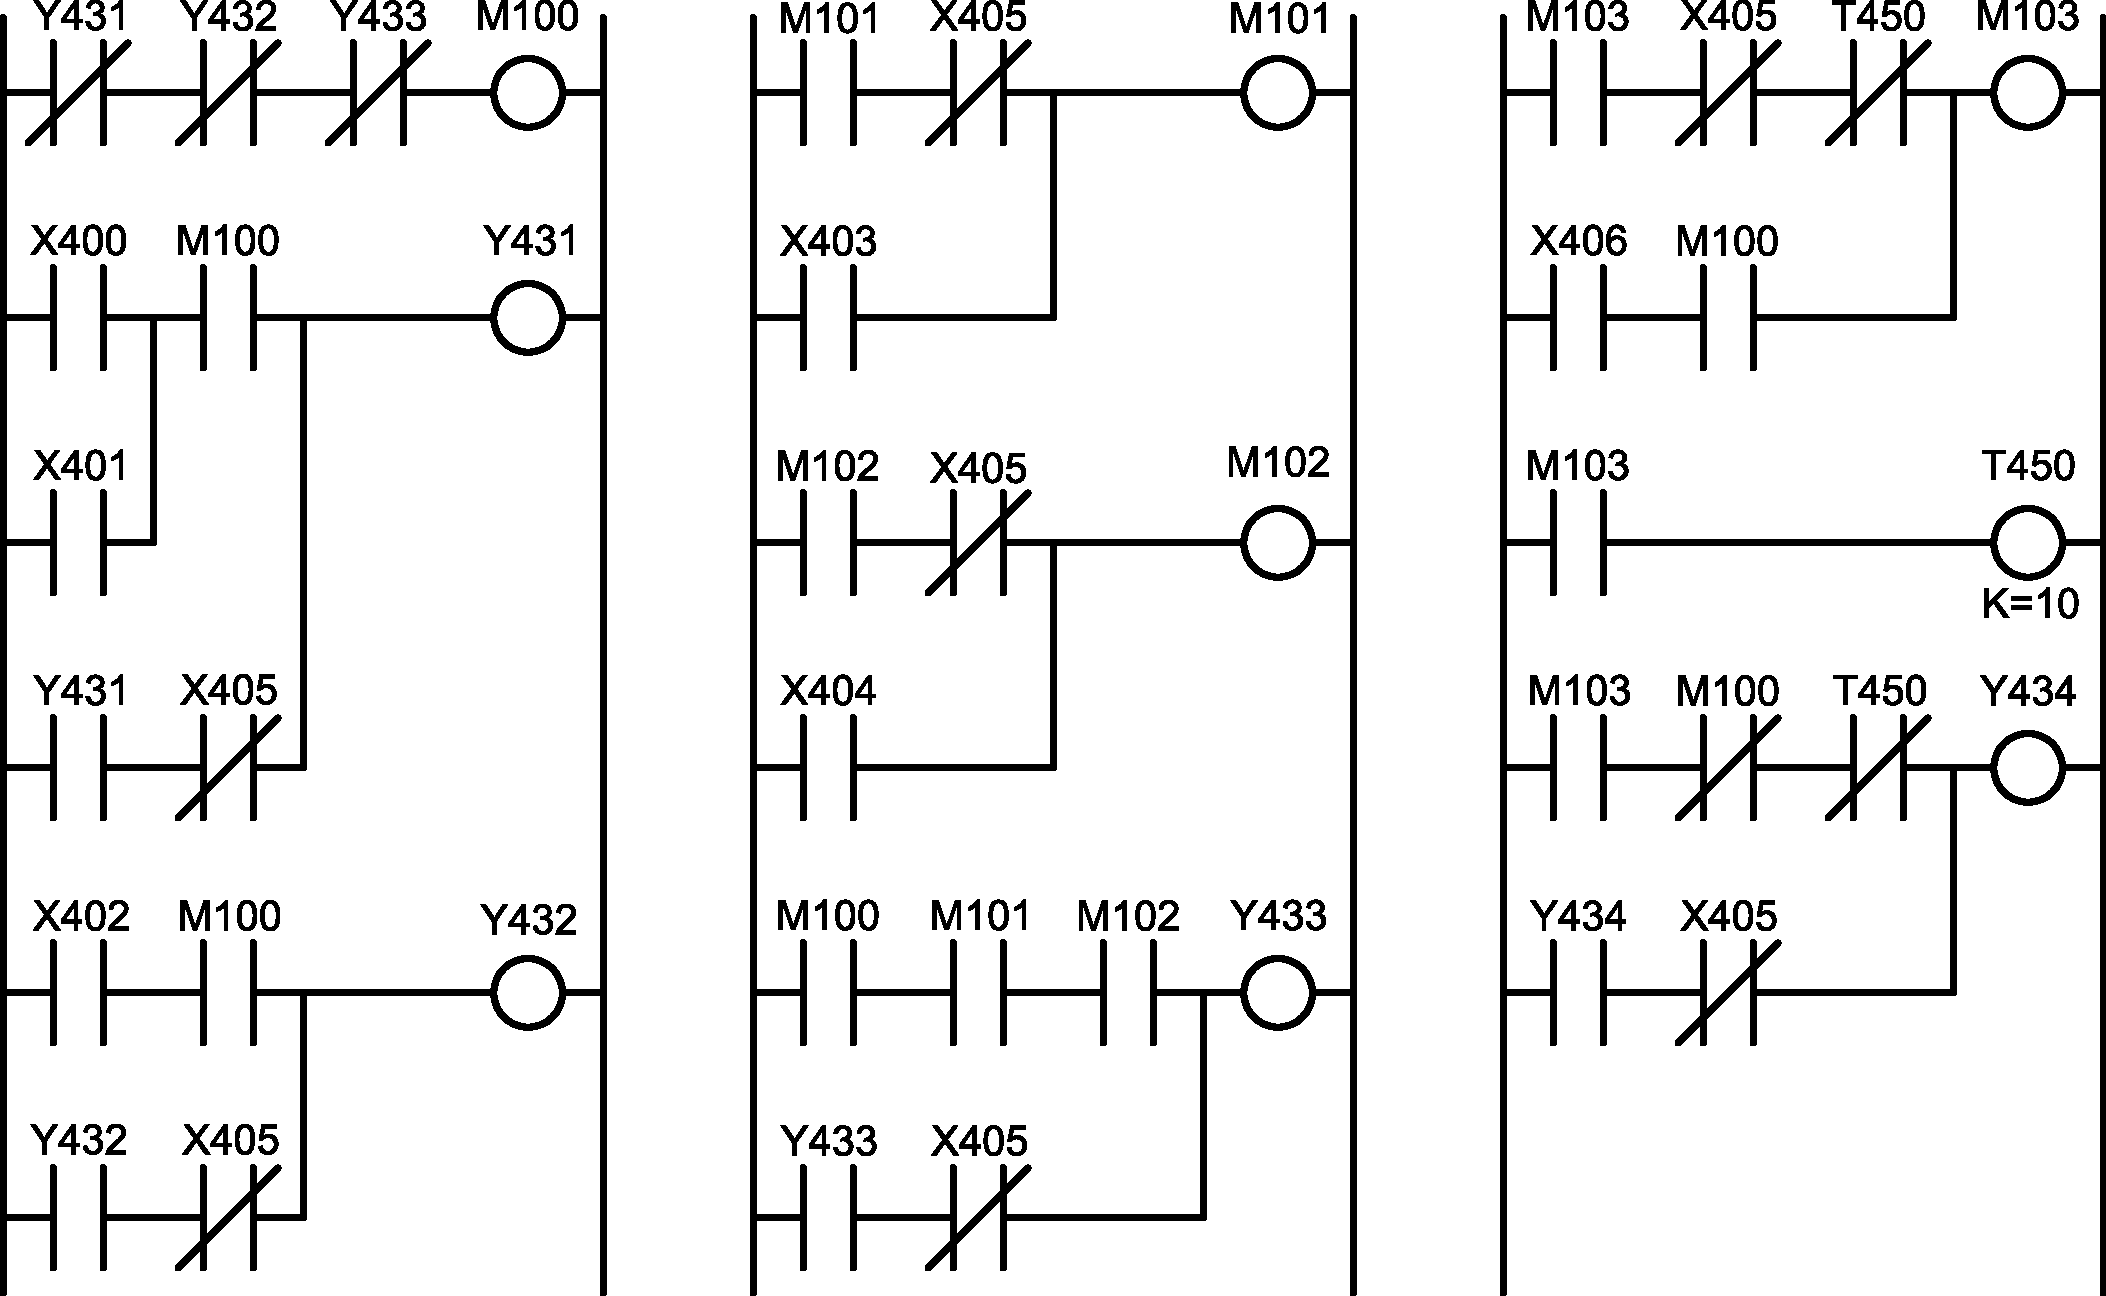
\includegraphics[width=14cm]{images/quiz_lad.pdf}
      \caption{リレーラダー図}
      \label{fig:quiz_lad}
    \end{figure}
    \begin{table}[h]
      \caption{コーディング}
      \label{tab:quiz_code}
      \centering
      \begin{tabular}{r|lr||r|lr||r|lr||r|lr||r|lr}
        0 & LDI & 431 & 10 & OUT & 431 & 20 & OUT & 101 & 30 & ORB & &     40 & OUT & 450 \\
        1 & ANI & 432 & 11 & LD &  402 & 21 & LD &  102 & 31 & OUT & 433 & 41 & K &   10 \\
        2 & ANI & 433 & 12 & AND & 100 & 22 & ANI & 405 & 32 & LD &  103 & 42 & LD &  103 \\
        3 & OUT & 100 & 13 & LD &  432 & 23 & OR &  404 & 33 & ANI & 405 & 43 & ANI & 100 \\
        4 & LD &  400 & 14 & ANI & 405 & 24 & OUT & 102 & 34 & ANI & 450 & 44 & ANI & 450 \\
        5 & OR &  401 & 15 & ORB & &     25 & LD &  100 & 35 & LD &  406 & 45 & LD &  434 \\
        6 & AND & 100 & 16 & OUT & 432 & 26 & AND & 101 & 36 & AND & 100 & 46 & ANI & 405 \\
        7 & LD &  431 & 17 & LD &  101 & 27 & AND & 102 & 37 & ORB & &     47 & ORB & \\
        8 & ANI & 405 & 18 & ANI & 405 & 28 & LD &  433 & 38 & OUT & 103 & 48 & OUT & 434 \\
        9 & ORB & &     19 & OR &  403 & 29 & ANI & 405 & 39 & LD &  103 & 49 & END & \\
      \end{tabular}
    \end{table}
\section{押しボタン式横断歩道の設計}
  今回の実験を通して新しくステップラダー方式を学ぶ.
  ステップラダー方式はリレーラダー方式と違い,
  状態遷移図に基づいてプログラムを作成する.
  この節では, 以下の制御仕様を満たすようにステップラダー方式を使ってプログラムを作成する.
  \subsection{制御仕様}
    \begin{itemize}
      \item 横断ボタンX400またはX401が押されると, 図\ref{fig:sig_pat}のパターンで信号灯が
        切り替わる. 一連の動作中に押しボタンを押しても無効とする.
      \item 設計には並進分岐のステップラダーを使用し, 点滅にはカウンタを使用する.
        使用するタイマーでは図の時間のみ使用する.
    \end{itemize}
    \begin{figure}[h]
      \centering
      % \includegraphics[]{}
      \caption{信号の動作パターン}
      \label{fig:sig_pat}
    \end{figure}
  \subsection{設計}
    まず, 入出力対応表を示す.
    \begin{table}[h]
      \caption{入出力対応表}
      \centering
      \begin{tabular}{c|c||c|c}
        \hline
        名前 &       シーケンサ & 名前 &         シーケンサ \\ \hline \hline
        押しボタン1 & X400 &     車用青信号 &    Y432 \\
        押しボタン2 & X401 &     歩行者用赤信号 & Y433 \\
        車用赤信号 &  Y430 &     歩行者用青信号 & Y434 \\
        車用黄信号 &  Y431 & & \\ \hline
      \end{tabular}
    \end{table}

    次に, 状態遷移図, ステップラダー図, コーディングを示す.
    \begin{figure}[h]
      \centering
      % includegraphics[]{}
      \caption{状態遷移図}
    \end{figure}
    \begin{figure}[h]
      \centering
      % includegraphics[]{}
      \caption{ステップラダー図}
    \end{figure}
    \begin{table}[h]
      \caption{コーディング}
      \label{tab:sig_code}
      \centering
      \begin{tabular}{r|lr||r|lr||r|lr||r|lr||r|lr}
        0 &  LD &  71 &  15 & STL & 601 & 30 & K &   5 &   45 & S &   607 & 60 & STL & 603 \\
        1 &  S &   600 & 16 & OUT & 432 & 31 & STL & 604 & 46 & STL & 607 & 61 & STL & 610 \\
        2 &  OUT & 671 & 17 & OUT & 450 & 32 & OUT & 433 & 47 & OUT & 434 & 62 & LD &  456 \\
        3 &  K &   601 & 18 & K &   30 &  33 & LD &  452 & 48 & OUT & 455 & 63 & S &   600 \\
        4 &  OUT & 672 & 19 & LD &  450 & 34 & S &   605 & 49 & K &   0.5 & 64 & RET & \\
        5 &  K &   610 & 20 & S &   602 & 35 & STL & 605 & 50 & LD &  455 & 65 & LD &  71 \\
        6 &  OUT & 670 & 21 & STL & 602 & 36 & OUT & 434 & 51 & AND & 460 & 66 & OR &  433 \\
        7 &  K &   103 & 22 & OUT & 431 & 37 & OUT & 453 & 52 & S &   606 & 67 & RST & 460 \\
        8 &  STL & 600 & 23 & OUT & 451 & 38 & K &   15 &  53 & LD &  455 & 68 & K &   5 \\
        9 &  OUT & 432 & 24 & K &   10 &  39 & LD &  453 & 54 & ANI & 460 & 69 & LD &  434 \\
        10 & OUT & 433 & 25 & LD &  451 & 40 & S &   606 & 55 & S &   610 & 70 & OUT & 460 \\
        11 & LD &  400 & 26 & S &   603 & 41 & STL & 606 & 56 & STL & 610 & 71 & END & \\
        12 & OR &  401 & 27 & STL & 603 & 42 & OUT & 454 & 57 & OUT & 433 & & & \\
        13 & S &   601 & 28 & OUT & 430 & 43 & K &   0.5 & 58 & OUT & 456 & & & \\
        14 & S &   604 & 29 & OUT & 452 & 44 & LD &  454 & 59 & K &   5 & & & \\
      \end{tabular}
    \end{table}
\section{課題}
  今回の実験を通して, リレーラダー方式とステップラダー方式の違いについて考えてみた.

  ステップラダー方式は状態遷移図をもとにプログラムを作成するので,
  一連の動作があるわけではない, 状態ごとに入力と動作があるプログラムに適している.
  今回の実験で作成した二つのプログラムはどちらもこれである.
  実際に, クイズの解答システムをステップラダー方式で設計してみると,
  リレーラダー方式で設計するよりも簡単にできる.

  逆に信号機のプログラムをリレーラダー方式で設計すると,
  とても手間がかかる.
  これは, 状態の概念をリレーラダー方式で管理すると,
  それぞれの状態に対応するフラグ出力を用意して,
  全ての入力に対してそのフラグと論理積を取って回路を組む必要があるからである.
\section{感想}
  今回のレポート作成において,
  表\ref{tab:quiz_code}, \ref{tab:sig_code}などのコーディングがとても手間がかかった.
  \LaTeX の表作成はそもそも手間がかかるが,
  今回のコーディングに関しては行番号があるので, 自動でインデクシングをしてくれる方法などが
  あればいいなと思った.
\section*{参考文献}
  \begin{enumerate}
    \item 令和元年度電子制御工学実験 $\cdot$ 3年後期テキスト
  \end{enumerate}
\end{document}
